\chapter{State of the Art}
\label{cha:state_of_art}

Single-molecule real-time- and nanopore sequencing are commonly referred to as third generation sequencing technologies.
Continuous improvements on platform, library preparation and analysis software still lead to throughput and accuracy enhancements.
Following latest developments in third generation sequencing is therefore equally important for both, users and developers.
The availability of significantly longer reads enables novel insights, published in a rapidly growing number of studies, making a systematic and unbiased manual literature research increasingly complex.
The following review is therefore backed by the computational evaluation of meta data from publications in scientific journals.
Combining title, abstract and citations into a literature graph opens a unique perspective and provides a scalable approach to sweep any number of publications.
In addition to the major application fields of assembly, structural variant and isoform detection, we find a largely separated landscape, either relying on Pacific Biosciences or Oxford Nanopore Technologies.
Supplementary code for this chapter is available at \textit{https://github.com/giesselmann/scholar}.

\begin{figure}[h]
	\centering
	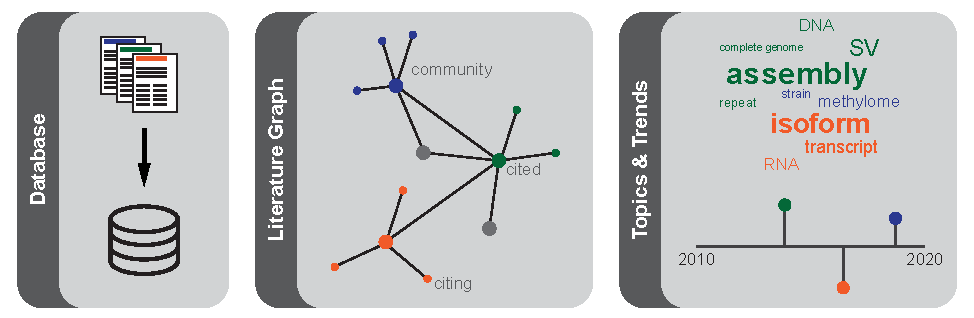
\includegraphics[width=1.0\textwidth]{figures/state_of_art/GA.pdf}
	\label{fig:state_of_art:ga}
\end{figure}

The chapter starts with a \textbf{background} in \ref{sec:state_of_art:background} followed by the setup and usage of a \textbf{literature database} containing scientific publication meta data in \ref{sec:state_of_art:database}. A big picture overview of \textbf{third generation sequencing} technologies in \ref{sec:state_of_art:third_generation}, is followed by a focus on \textbf{nanopore sequencing} in \ref{sec:state_of_art:nanopore}. Finally, most recent \textbf{throughput and accuracy} benchmarks on in-house data close the state of the art evaluation.




\section{Background}
\label{sec:state_of_art:background}

The number of studies published per year in scientific journals is exponentially growing (Fig. \ref{fig:state_of_art:paper_count}).
Including only records with a digital object identifier (DOI) tracked by CrossRef and Semantic Scholar, results in a conservative estimation of 100k journals and a total of 5M paper being published only in 2020.
While the targeted discovery of specific studies remains feasible by indexing in search engines, the extensive and continuous tracking of an entire field of research becomes increasingly difficult.
Especially for the fast evolving field of nanopore sequencing, a zoomed out perspective is equally valuable for the orientation of newcomers and adaptation to latest developments in experienced groups.
A data driven literature scan facilitates the clustering of results and identification of key publications in an unbiased way.

%Zoom out history \cite{Deamer2016}

\begin{figure}[h]
	\centering
	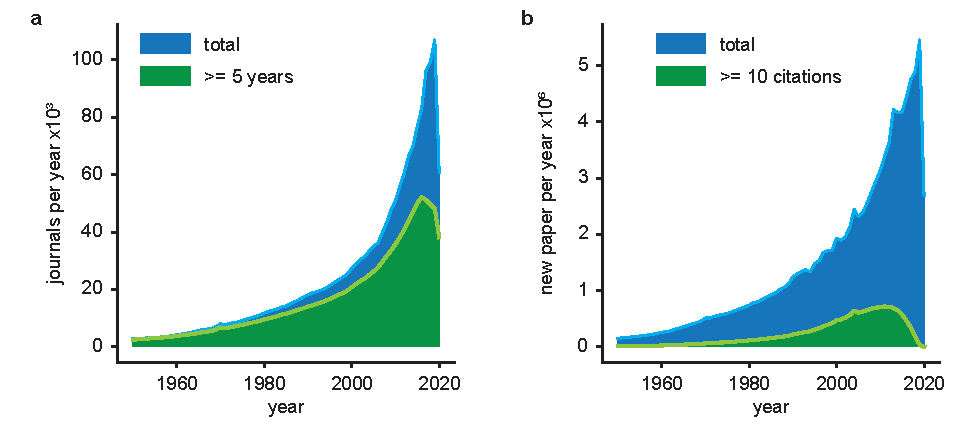
\includegraphics[width=1.0\textwidth]{figures/state_of_art/paper_count.pdf}
	\captionsetup{format=plain}
	\caption[Journals and publications per year]{Journals and new publications per year: \textbf{a}, Actively publishing scientific journals per year and journals with a history of at least five years. \textbf{b}, New publications per year and publications with at least 10 citations. (Semantic Scholar and CrossRef combined, only records with DOI)}
	\label{fig:state_of_art:paper_count}
\end{figure}

The following computer aided literature analysis is inspired by the Open Syllabus Galaxy\footnote{\url{https://galaxy.opensyllabus.org/}, accessed 01/2021} project.
Based on co-assignments of books in North American university courses, their literature graph of 160k books visualizes the linkage between research fields.
Applied to scientific journal publications, the success of the method is limited by the availability and quality of large scale meta data such as title, abstract and citations.
A number of platforms like Google Scholar, Web of Science, Dimensions or Microsoft Academic operate online literature databases, though without access to larger data chunks for systematic offline analysis.
Additional full text for advanced text mining is commonly only available through paid access from individual journals.




\section{Literature Database}
\label{sec:state_of_art:database}

For the purpose of tracing citations and clustering larger numbers of publications, we first setup a custom literature database.
The Semantic Scholar open research corpus (S2ORC) provides the largest available collection of scientific paper meta data and serves as starting point in this work \cite{Lo2020}.
Collected 07/2020, the data contains 77M papers linked by 333M citations.
Provided as compressed JSON files, the records are re-organized into a SQLite database with two main tables for records and citations.
Each record is uniquely identified by it's DOI and can additionally contain year, journal, title and abstract.
Citations are unique pairs of citing and cited DOI, referencing rows in the records table.
To further improve completeness of records and citations, we incrementally query the CrossRef REST API\footnote{\url{https://github.com/CrossRef/rest-api-doc}, accessed 01/2021} for novel entries, most recently in January 2021.
Citations are part of CrossRef but not provided through the API.
The CrossRef Open Citations Index (COCI) however, is regularly parsing and dumping citations and therefore integrated as well \cite{Peroni2020}.
Metrics of the final database used for this work are summarized in table \ref{tab:state_of_art:graph}. 
For comparison, the Dimensions\footnote{'url{https://www.dimensions.ai/}, accessed 01/2021} online platform lists 114M records and 1.3G citations.

\begin{table}[ht]
	\centering
	\caption[Literature Graph Metrics]{Literature database metrics}
	\label{tab:state_of_art:graph}
	\begin{tabular}{l|r}
		\hline
		citations (edges)           & 901 M 	\\
		paper (nodes)               & 116 M 	\\ \hline
		with title					& 115 M		\\
		with title \& abstract		&  57 M		\\ \hline
		connected nodes             &  68.4 M 	\\
		> 0 citations				&  56.6 M	\\
		> 5 citations				&  27.5 M	\\
		largest connected component &  67.9 M 	\\ \hline
	\end{tabular}
\end{table}

The network of publications and citations can also be interpreted as a literature graph with papers as nodes and citations as edges.
Only a fraction of 68M publications has either citing or cited edges.
The lack of citing (outgoing) edges indicates insufficient parsing of the papers reference sections, while the lack of cited (incoming) edges is likely a combination of technical limitations and unrecognized publications.
Striking though, is the presence of the largest connected component of 67.9M publications, where each paper can be reached via at least one citation edge.

A subset of publications originating from the S2ORC data set is annotated with a primary field of research from Microsoft Academic (MA). 
To get a first impression of the value of a literature graph, we extract all edges connecting papers with an annotated field of research.
A hierarchical clustering of summarized citation counts per field is plotted as heatmap in Fig. \ref{fig:state_of_art:field_interactions}, and shows an intuitive grouping of natural- and social sciences.

\begin{figure}[h]
	\centering
	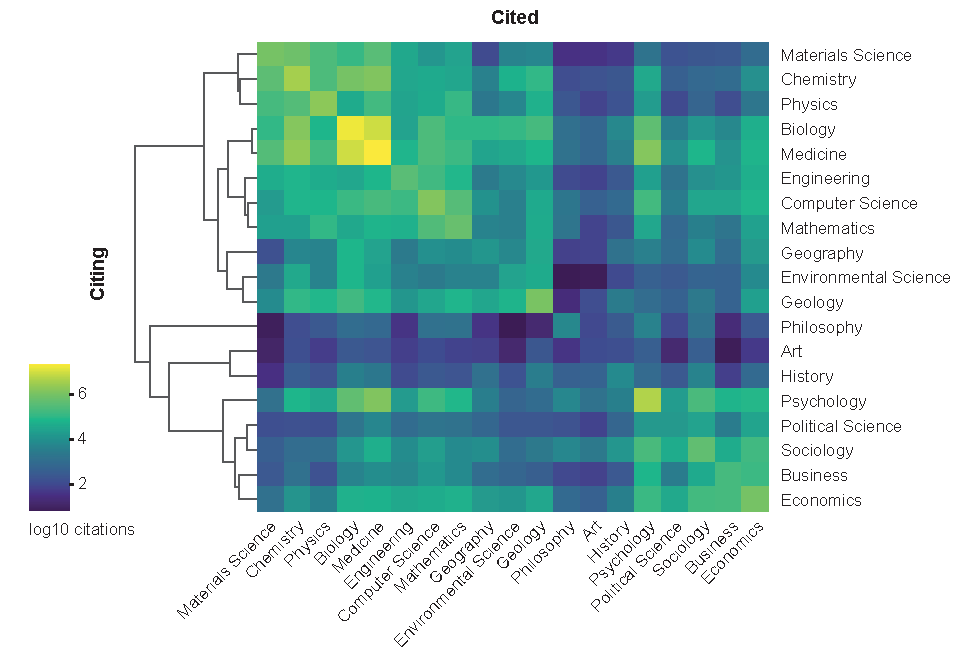
\includegraphics[width=1.0\textwidth]{figures/state_of_art/field_interactions.pdf}
	\captionsetup{format=plain}
	\caption[Scientific field interactions]{Citation edges summarized by field of research: Sum of citations (log10) between and within fields of research (Hierarchical clustering, method: centroid, distance: cosine).}
	\label{fig:state_of_art:field_interactions}
\end{figure}

A graph is a powerful data structure, for instance to detect local communities or compute distances between nodes, however, with a growing number of nodes and edges it becomes impossible to visualize.
For the purpose of visualization and clustering, a graph embedding, similar to the \textit{node2vec} algorithm used in the OpenSyllabus project is therefore needed \cite{Grover2016}.
A graph embedding is a fixed length vector representation of each node, with the aim to preserve local connectivity.
The vector representation is enabling distance based clustering methods such as KMeans and dimensional reduction by principal component analysis (PCA) and uniform manifold approximation (UMAP).
Additionally, while sub-sampling nodes of a graph would split connected components, sub-sampling from an embedded graph, based on e.g. citation counts or topic, preserves the overall structure and reduces required compute resources.

Embedding the scientific literature graph using \textit{node2vec} is due to run-times of multiple weeks on CPU and large memory requirements on GPU not feasible.
We use therefore the \textit{DeepWalk} \cite{Perozzi2014} algorithm with its GPU implementation in \textit{GraphVite} \cite{Zhu2019}.
In order to fit on a GPU-server with 4x NVIDIA 2080Ti (11 GB RAM), only edges connecting publications with at least 20 citations are considered.
The resulting sub-graph, in the following referred to as \textbf{core\_20} graph, contains 9M nodes with virtually a single connected component.

Embedding with default parameters yields feature vectors of length 128 for each publication.
Following the OpenSyllabus projects workflow, a high-level visualization is generated by first reducing to 64 dimensions using PCA (85\% explained variance), followed by further reduction to two dimensions using a UMAP.

\begin{figure}[h]
	\centering
	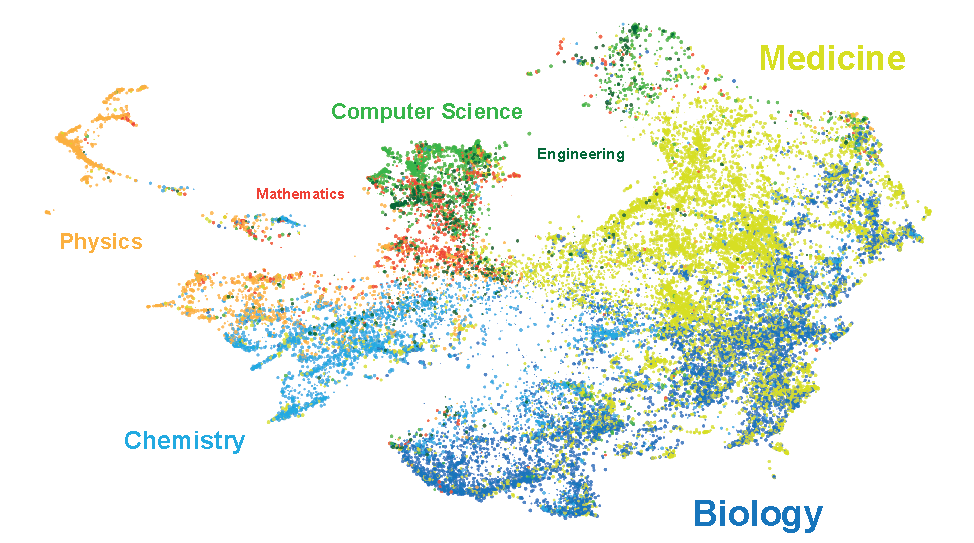
\includegraphics[width=1.0\textwidth]{figures/state_of_art/umap_global.pdf}
	\captionsetup{format=plain}
	\caption[Scientific literature graph]{Scientific publication graph embedding: UMAP visualization of \textit{DeepWalk} graph embedding colored by field of research. Publications from 1980 onward with at least 20 citations (n=9M embedded, n\_neighbors 75, min\_dist 0.01, metric correlation, n=50k random sample plotted).}
	\label{fig:state_of_art:umap_global}
\end{figure}




\section{Third Generation Sequencing}
\label{sec:state_of_art:third_generation}

PacBio seed 2900, nanopore seed 2852.
Compare to Dimensions: 3147 publications for 'nanopore AND sequencing' (01/2021)
While the PacBio and Nanopore cluster grow to similar sizes of 6159 and 6085 publications respectively, the number of nodes reached by both extensions is only 492.


\begin{figure}[h]
	\centering
	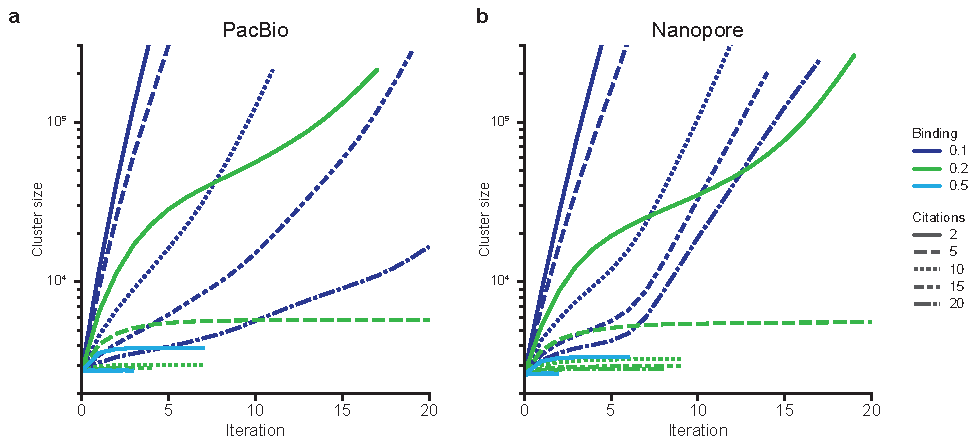
\includegraphics[width=1.0\textwidth]{figures/state_of_art/cluster_convergence.pdf}
	\captionsetup{format=plain}
	\caption[Keyword Seed and Extend Convergence]{Cluster size convergence for keyword seed and extend strategy.}
	\label{fig:state_of_art:cluster_convergence}
\end{figure}

Intersection with core network 1980/20 citations is 0.10 for PacBio and 0.17 for nanopore.
Not all seed nodes have citations, long read cluster of pacbio and nanopore contains 10k nodes from 142 connected components, however the largest cc is 9492.
21 connected components have at least one overlap into 20 citations backbone graph.

After backbone expansion, 43051 nodes with largest cc 42638
Same embedding as above, complemented with random walks from core\_20 backbone citations. Mostly separated, disconnected nanopore cluster, some interleaved areas.

\begin{figure}[h]
	\centering
	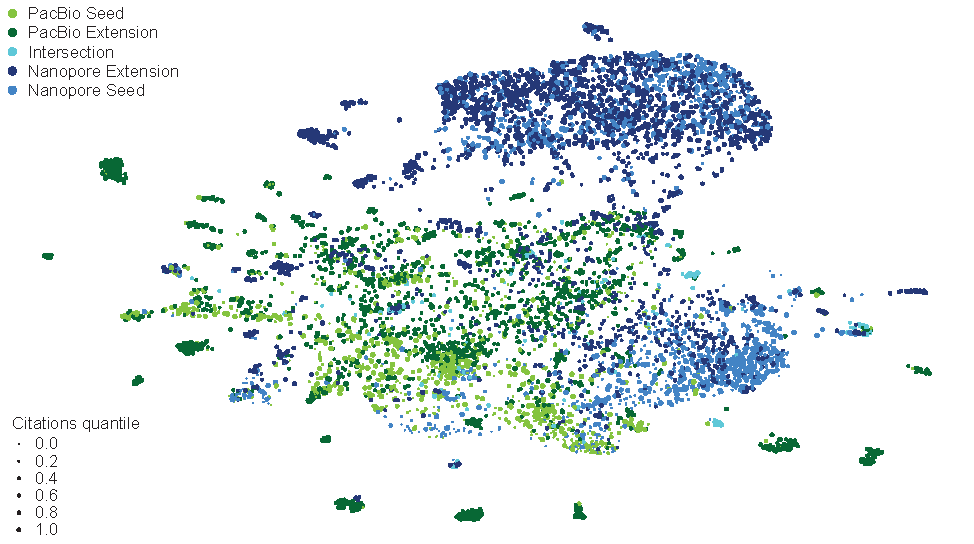
\includegraphics[width=1.0\textwidth]{figures/state_of_art/umap_lr.pdf}
	\captionsetup{format=plain}
	\caption[Third generation sequencing cluster]{Third generation sequencing cluster}
	\label{fig:state_of_art:umap_lr}
\end{figure}

Hierarchical clustering of cluster centers, publication year distribution and seed to extension composition of clusters.

\begin{figure}[h]
	\centering
	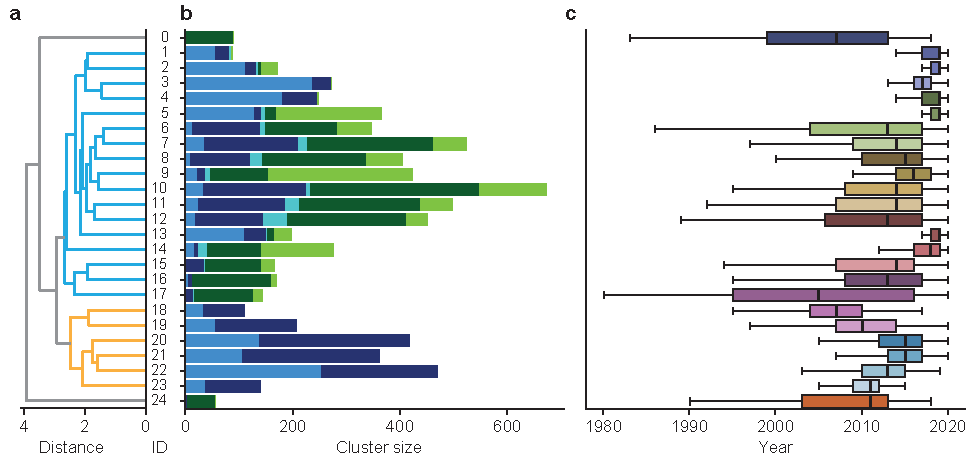
\includegraphics[width=1.0\textwidth]{figures/state_of_art/cluster_sizes.pdf}
	\captionsetup{format=plain}
	\caption[Long-Read Application Cluster]{Cluster of long-read applications:}
	\label{fig:state_of_art:cluster_sizes}
\end{figure}

Extract most variant keyword tokens by TF-IDF embedding and generate word clouds of tokens with high inter-cluster variance.

\begin{figure}[h]
	\centering
	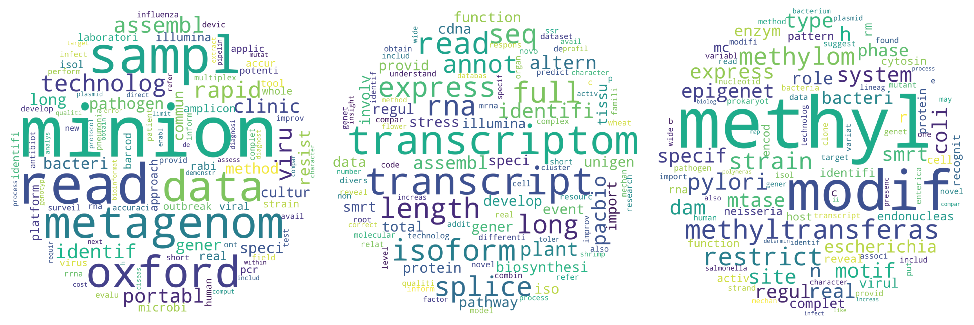
\includegraphics[width=1.0\textwidth]{figures/state_of_art/wcs_minion.pdf}
	\captionsetup{format=plain}
	\caption[Nanopore Sequencing Wordclouds]{Nanopore sequencing word clouds of cluster 2, 3 and 5.}
	\label{fig:state_of_art:wcs_minion}
\end{figure}

\begin{figure}[h]
	\centering
	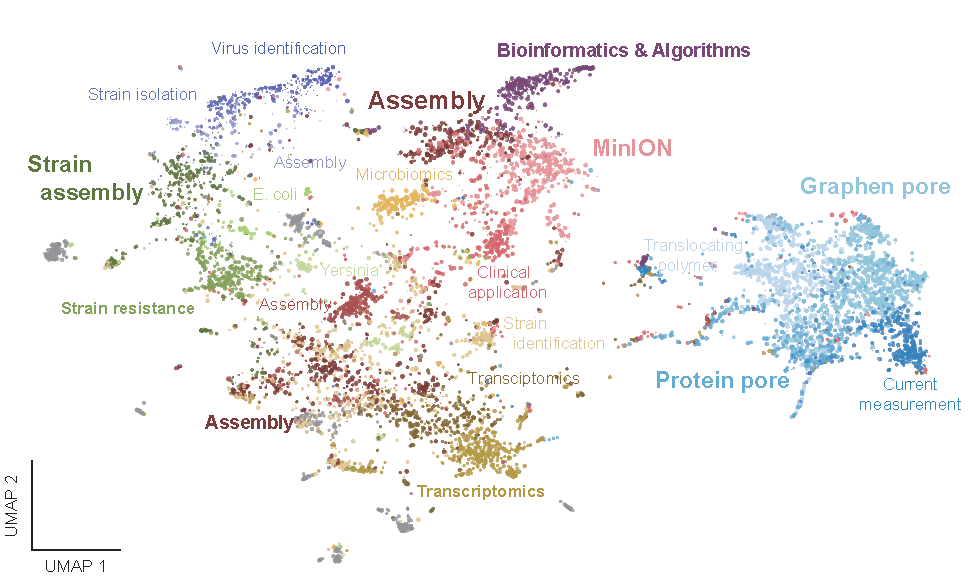
\includegraphics[width=1.0\textwidth]{figures/state_of_art/umap_cluster.pdf}
	\captionsetup{format=plain}
	\caption[Third generation sequencing cluster]{Third generation sequencing cluster}
	\label{fig:state_of_art:umap_cluster}
\end{figure}

PacBio methylation whitepaper \footnote{\url{https://www.pacb.com/wp-content/uploads/2015/09/WP_Detecting_DNA_Base_Modifications_Using_SMRT_Sequencing.pdf}, accessed 01/2021}:
25X for 6mA but 250X for 5mC and 5hmC


\subsection{Nanopore Development}
\label{subsec:state_of_art:nanopore}

\subsection{Bacterial Strain}
\label{subsec:state_of_art:strain}

\subsection{Assembly}
\label{subsec:state_of_art:assembly}

\subsection{Isoform Detection}
\label{subsec:state_of_art:isoform}

PacBio 4M reads per smart cell
Nanopore 5-10M for cDNA kit, 1M direct RNA kit

\subsection{Epigenetics}
\label{subsec:state_of_art:epigenetics}




\section{Focus Nanopore Sequencing}
\label{sec:state_of_art:nanopore}




%\section{\Biorxiv\ Preprints}
%\label{sec:state_of_art:biorxiv}




\section{Throughput and Accuracy}
\label{sec:stat_of_art:throughput}

\begin{itemize}
    \item Representative Flow-Cells over time (from 3 to 30 GBp in 48h)
    \item Size selection, shearing, nuclease flush
    \item accuracy guppy-fast, guppy-hac (mention albacore flappie, scrappie, SACall, chiron, ...)
    \item cite benchmark paper, illustrate need for in-house benchmark of each new version
    \item Mapping of long reads depending on genomic context, read length, Q-Score etc.
    \item Accuracy of base modifications: Nanopolish, Signalign, DeepMod, DeepSignal etc.
    %\item Nanopolish context and signal level analysis
\end{itemize}

\begin{figure}[h]
    \centering
    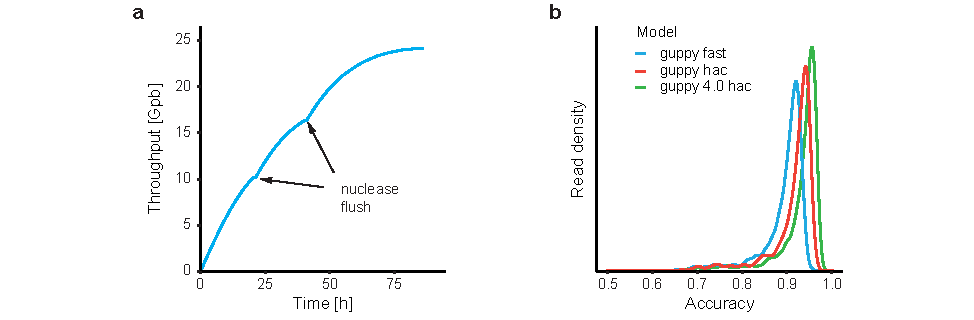
\includegraphics[width=1.0\textwidth]{figures/state_of_art/throughput.pdf}
    \captionsetup{format=plain}
    \caption[Throughput and accuracy]{Throughput and single read accuracy. \textbf{a}, Cumulative sequencing throughput over time of one representative MinION flow cell. Nuclease flushes unblock clogged pores and reload the flow cell with a new library. \textbf{b}, Density plot comparing single read accuracy (BLAST identiy) of 4k random reads basecalled with fast and high-accuracy model of \textit{Guppy} v3.5 and high-accuracy model of \textit{Guppy} v4.0 (Median accuracy: 0.90, 0.93, 0.95; Modal: 0.92, 0.94, 0.95).}
    \label{fig:state_of_art:throughput}
\end{figure}

\begin{figure}[h]
    \centering
    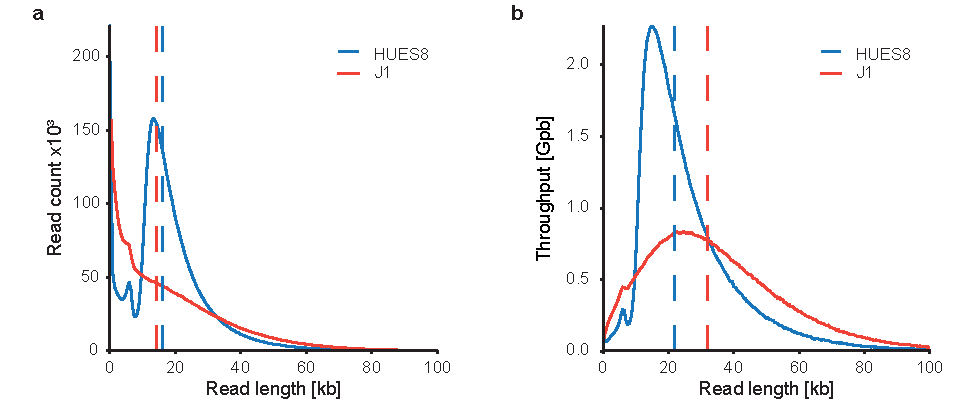
\includegraphics[width=1.0\textwidth]{figures/state_of_art/read_length.pdf}
    \captionsetup{format=plain}
    \caption[Read length median and N50]{Read length distribution: \textbf{a}, Read length distributions shown as number of reads per length (bins of 500nt) of two PromethION flow cells loaded with libraries from different DNA extraction methods. Dashed lines show median read length at 15883 (HUES8) and 14281 (J1). \textbf{b}, Read length distributions shown as sequenced basepairs per read length. Dashed lines show N50 at 21041 (HUES8) and 31906 (J1).}
    \label{fig:state_of_art:read_length}
\end{figure}

\begin{figure}[h]
    \centering
    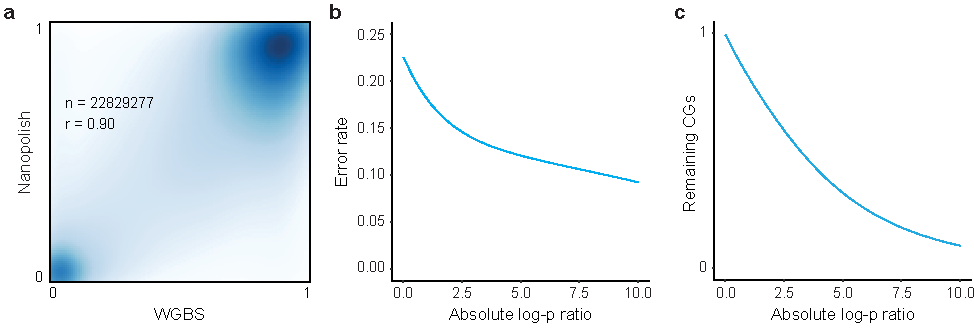
\includegraphics[width=1.0\textwidth]{figures/state_of_art/methylation.pdf}
    \captionsetup{format=plain}
    \caption[Nanopore methylation detection]{Nanopore 5mC methylation detection: \textbf{a}, Correlation of whole genome bisulfite sequencing (WGBS) and nanopore sequenced mean methylation rates per genomic position (\textit{Nanopolish} detection with abs. log-p threshold: 2.5, min. coverage: 10X, reference hg19). \textbf{b}, Detection error depending on the applied absolute log-likelihood ratio (methylation probability) threshold. \textbf{c}, Fraction of dataset remaining depending on log-p value threshold.}
    \label{fig:state_of_art:methylation}
\end{figure}




\section{Summary}
\label{sec:stat_of_art:summary}








